%=============================================================================%
% Author: 	John Joseph Valletta
% Date: 	23/04/2017
% Title: 	Python workshop: Pandas
%=============================================================================%

%=============================================================================%
% Preamble
%=============================================================================%
% Libraries
\documentclass[pdf]{beamer}
\usepackage[export]{adjustbox}
\usepackage{framed}
\usepackage{color}
\definecolor{dkgreen}{rgb}{0,0.6,0}
\definecolor{gray}{rgb}{0.5,0.5,0.5}
\definecolor{mauve}{rgb}{0.58,0,0.82}
\definecolor{deepblue}{rgb}{0,0,0.5}
\definecolor{deepred}{rgb}{0.6,0,0}
\definecolor{deepgreen}{rgb}{0,0.5,0}
\definecolor{lightgray}{rgb}{0.92,0.92,0.92}
\usepackage{listings} % to insert code
\usepackage{textpos} % textblock
\usepackage{dirtree} % to make directory trees
\usepackage{hyperref}
\hypersetup{colorlinks=true, urlcolor=blue, linkcolor=black} 

% Listing set up
% Python
\lstdefinestyle{python}{
language=python,
formfeed=\newpage,
basicstyle=\scriptsize\ttfamily,
commentstyle=\color{deepgreen},%\color{gray},
%numbers=left,
%numberstyle=\tiny\color{gray},
stepnumber=1,
numbersep=5pt,
backgroundcolor=\color{lightgray},%\color{white},
showspaces=false,
showstringspaces=false,
showtabs=false,
frame=lines,
tabsize=4,
captionpos=b,
breaklines=true,
breakatwhitespace=false,
title=\lstname,
escapeinside={},
keywordstyle=\color{deepblue},
emphstyle=\color{deepred},
stringstyle=\color{mauve},
morekeywords={as, lambda}
}

% Presentation configuration
\mode<presentation>{\usetheme{Madrid}}
\definecolor{tealblue}{rgb}{0, 0.5, 0.5}
\usecolortheme[named=tealblue]{structure}
\useinnertheme{circles} % circles, rectanges, rounded, inmargin
\usefonttheme[onlymath]{serif} % makes math fonts like the usual LaTeX ones
\setbeamercovered{transparent=4} % transparent
\setbeamertemplate{caption}{\raggedright\insertcaption\par} % Remove the word "Figure" from caption %\setbeamertemplate{caption}[default]
\setbeamertemplate{navigation symbols}{} % don't put navigation tools at the bottom (alternatively \beamertemplatenavigationsymbolsempty)
\graphicspath{ {../images/} }

% Titlepage
\title[Python for scientific research]{Python for scientific research}
\subtitle{Data analysis with \texttt{Pandas}}
\author{John Joseph Valletta}
\date[June 2017]{June 2017}
\institute[]{University of Exeter, Penryn Campus, UK}
\titlegraphic{
\hfill

\includegraphics[width=\textwidth, keepaspectratio]{logo.jpg}}

%=============================================================================%
%=============================================================================%
% Start of Document
%=============================================================================%
%=============================================================================%
\begin{document}

%=============================================================================%
%=============================================================================%
\begin{frame}
\titlepage
\end{frame}

%=============================================================================%
%=============================================================================%
\begin{frame}{What we've done so far}

	\begin{enumerate}\addtolength{\itemsep}{.7\baselineskip}
		\item Declare variables using built-in data types and execute operations
		on them
		\item Use flow control commands to dictate the order in which commands are run
		and when
		\item Encapsulate programs into reusable functions, modules and packages
		\item Using \texttt{NumPy} and \texttt{SciPy} for numerical computations
		\item Produce publication-ready plots using \texttt{Matplotlib} 
		\item \textbf{Next}: Introducing \texttt{Pandas}, Python's library
		for data manipulation and analysis
	\end{enumerate}

\end{frame}

%=============================================================================%
%=============================================================================%
\begin{frame}{Introduction}

\texttt{Pandas} is Python's data analysis toolkit, used for:

\begin{itemize}\addtolength{\itemsep}{.5\baselineskip}
	\item<2-> Reading/writing data of different formats (e.g CSV, SQL database)
	\item<3-> Creating and manipulating data frames (akin to R)
	\item<4-> Handling missing data
	\item<5-> Meging/joining data sets
	\item<6-> Reshaping/pivoting data sets
	\item<7-> Time-series analysis
	\item<8-> $\ldots$
\end{itemize}

\end{frame}

%=============================================================================%
%=============================================================================%
\begin{frame}{Pandas data structures}

\begin{enumerate}
	\item \texttt{Series}
	\begin{itemize}
		\item A one dimensional object
		\item Similar to a list or array
		\item Each entry has a unique index
		\item Useful for time-series analysis
	\end{itemize}
\end{enumerate}

\begin{center}
	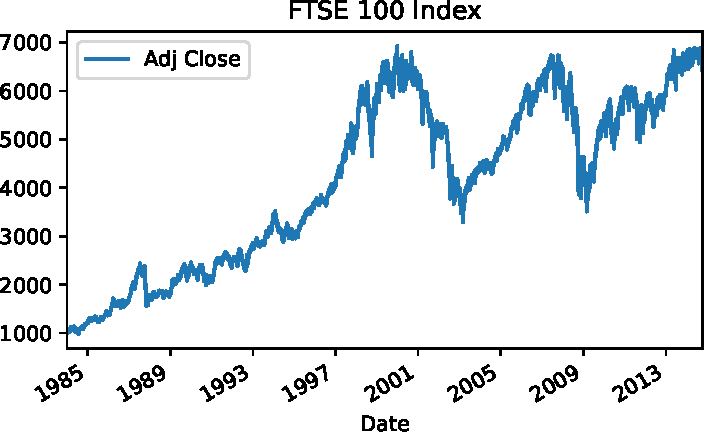
\includegraphics[width=.7\textwidth]{ftse1.pdf}
\end{center}

\end{frame}

%=============================================================================%
%=============================================================================%
\begin{frame}{Pandas data structures}

\begin{enumerate}
	\setcounter{enumi}{1}
	\item \texttt{DataFrame}
	\begin{itemize}
		\item A two dimensional object to store data
		\item Like a spreadsheet with rows and columns (akin to R's \texttt{data.frame})
		\item Each column is a \texttt{Pandas Series}
		\item Each row has a unique index
		\item Useful for any kind of data wrangling and analysis
	\end{itemize}
\end{enumerate}

\begin{center}
	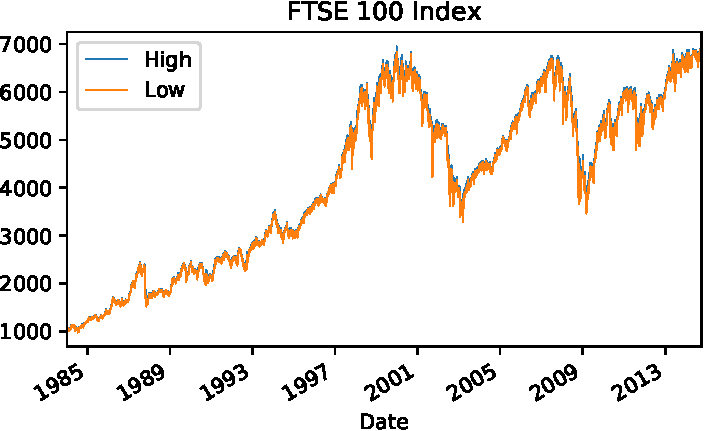
\includegraphics[width=.7\textwidth]{ftse2.pdf}
\end{center}

\end{frame}

%=============================================================================%
%=============================================================================%
\begin{frame}[fragile]
\frametitle{Create a \texttt{DataFrame}}

\begin{lstlisting}[style=python]
import pandas as pd

df = pd.DataFrame(
        {"Sample" : ["R100" , "R201", "R203", "R340", "R453"],
         "t0" : [0.2, 0.1, 0.3, 0.25, 0.13], 
         "t1" : [1.3, 1.8, 0.8, 1.5, 0.6],
         "t2" : [2.8, 3.1, 1.9, 2.3, 1.8],
         "t3" : [3.2, 3.7, 2.3, 3.5, 2.5],
         "t4" : [1.2, 1.8, 3.9, 1.3, 3.7],
         "t5" : [0.7, 0.4, 3.4, 0.3, 3.6]})

df.shape # return size of data set (5, 7)
\end{lstlisting}

\vspace{-0.8cm}

\footnotesize
\begin{verbatim}
  Sample    t0   t1   t2   t3   t4   t5
0   R100  0.20  1.3  2.8  3.2  1.2  0.7
1   R201  0.10  1.8  3.1  3.7  1.8  0.4
2   R203  0.30  0.8  1.9  2.3  3.9  3.4
3   R340  0.25  1.5  2.3  3.5  1.3  0.3
4   R453  0.13  0.6  1.8  2.5  3.7  3.6
\end{verbatim}
\normalsize

\end{frame}

%=============================================================================%
\begin{frame}[fragile]
\frametitle{Reshaping data}

\begin{lstlisting}[style=python]
# Gather time columns [t0,...,t5] into rows
df = pd.melt(df, 
             id_vars="Sample", 
             var_name="Time",
             value_name="Exprs")
\end{lstlisting}

\vspace{-0.8cm}

{\fontsize{5}{5}\selectfont
\begin{verbatim}
   Sample Time  Exprs
0    R100   t0   0.20
1    R201   t0   0.10
2    R203   t0   0.30
3    R340   t0   0.25
4    R453   t0   0.13
5    R100   t1   1.30
6    R201   t1   1.80
7    R203   t1   0.80
8    R340   t1   1.50
9    R453   t1   0.60
10   R100   t2   2.80
11   R201   t2   3.10
12   R203   t2   1.90
13   R340   t2   2.30
14   R453   t2   1.80
15   R100   t3   3.20
16   R201   t3   3.70
17   R203   t3   2.30
18   R340   t3   3.50
19   R453   t3   2.50
20   R100   t4   1.20
21   R201   t4   1.80
22   R203   t4   3.90
23   R340   t4   1.30
24   R453   t4   3.70
25   R100   t5   0.70
26   R201   t5   0.40
27   R203   t5   3.40
28   R340   t5   0.30
29   R453   t5   3.60
\end{verbatim}}

\end{frame}

%=============================================================================%
\begin{frame}[fragile]
\frametitle{Reshaping data}

\begin{lstlisting}[style=python]
# Spread rows into columns [by time]
df = pd.pivot_table(df,
                    values="Exprs", 
                    columns="Sample", 
                    index="Time")
\end{lstlisting}

\begin{verbatim}
Sample  R100  R201  R203  R340  R453
Time                                
t0       0.2   0.1   0.3  0.25  0.13
t1       1.3   1.8   0.8  1.50  0.60
t2       2.8   3.1   1.9  2.30  1.80
t3       3.2   3.7   2.3  3.50  2.50
t4       1.2   1.8   3.9  1.30  3.70
t5       0.7   0.4   3.4  0.30  3.60
\end{verbatim}

\end{frame}

%=============================================================================%
\begin{frame}[fragile]
\frametitle{Plot samples R100 and R453}

\begin{lstlisting}[style=python]
# Time-plot
df.plot(y=["R100", "R453"])

# Box-plot
df.plot(y=["R100", "R453"], kind="box")
\end{lstlisting}

\begin{center}
	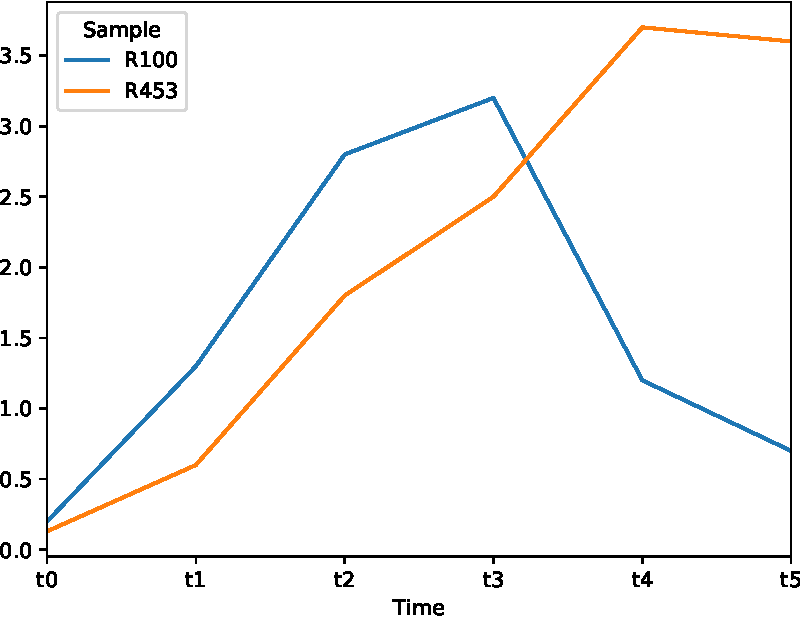
\includegraphics[width=.48\textwidth]{gene_exprs1.pdf}\hfill
	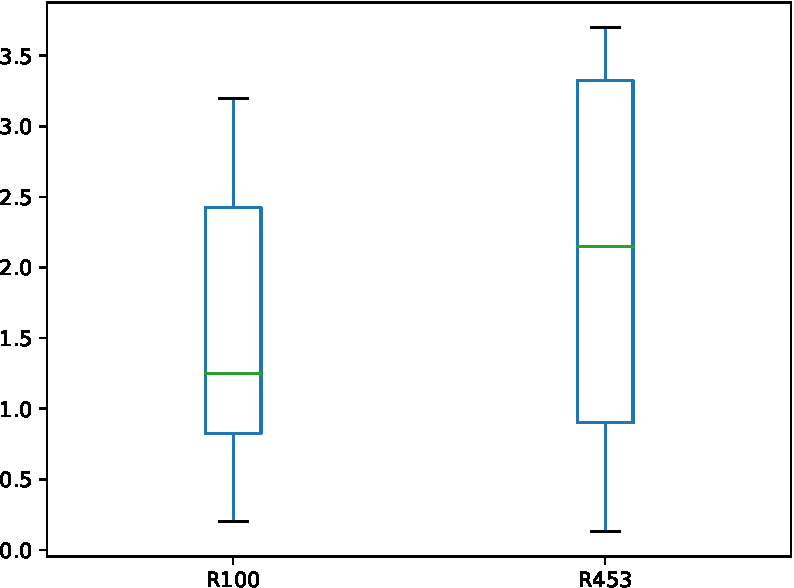
\includegraphics[width=.48\textwidth]{gene_exprs2.pdf}
\end{center}

\end{frame}

%=============================================================================%
%=============================================================================%
\begin{frame}[fragile]
\frametitle{Reading data files: Births per women}

\begin{lstlisting}[style=python]
# Read data file
data = pd.read_csv("births_per_woman.csv", header=0)

# Explore what's in the data 
data.head() # show first 5 rows of data
data.tail() # show last 5 rows of data
\end{lstlisting}

\vspace{-0.8cm}
{\fontsize{5}{6}\selectfont
\begin{verbatim}
   CountryName                     Region          IncomeGroup   1960   1961  \
0        Aruba  Latin America & Caribbean          High income  4.820  4.655   
1  Afghanistan                 South Asia           Low income  7.450  7.450   
2       Angola         Sub-Saharan Africa  Upper middle income  7.379  7.388   
3      Albania      Europe & Central Asia  Upper middle income  6.489  6.401   
4      Andorra      Europe & Central Asia          High income    NaN    NaN   

    1962   1963   1964   1965   1966  ...     2006   2007   2008   2009  \
0  4.471  4.271  4.059  3.842  3.625  ...    1.754  1.741  1.728  1.716   
1  7.450  7.450  7.450  7.450  7.450  ...    6.639  6.437  6.218  5.985   
2  7.396  7.402  7.406  7.408  7.406  ...    6.671  6.619  6.559  6.492   
3  6.282  6.133  5.960  5.773  5.581  ...    1.668  1.635  1.625  1.636   
4    NaN    NaN    NaN    NaN    NaN  ...    1.240  1.180  1.250  1.190   

    2010   2011   2012   2013   2014   2015  
0  1.704  1.692  1.680  1.669  1.657  1.647  
1  5.746  5.506  5.272  5.050  4.843  4.653  
2  6.416  6.335  6.251  6.165  6.080  5.996  
3  1.663  1.699  1.735  1.765  1.784  1.793  
4  1.270    NaN    NaN    NaN    NaN    NaN 
\end{verbatim}}

\end{frame}

%=============================================================================%
%=============================================================================%
\begin{frame}[fragile]
\frametitle{Descriptive statistics}

\begin{lstlisting}[style=python]
# Median births per woman 1970 vs 1990 vs 2010
data["1970"].median() # 5.7 births per woman
data["1990"].median() # 3.6 births per woman 
data["2010"].median() # 2.4 births per woman

# Box plot
data.plot(kind="box", rot=90, color={"medians": "red"}, 
          medianprops={"linewidth": 3})
\end{lstlisting}

\vspace{-0.6cm}
\begin{center}
	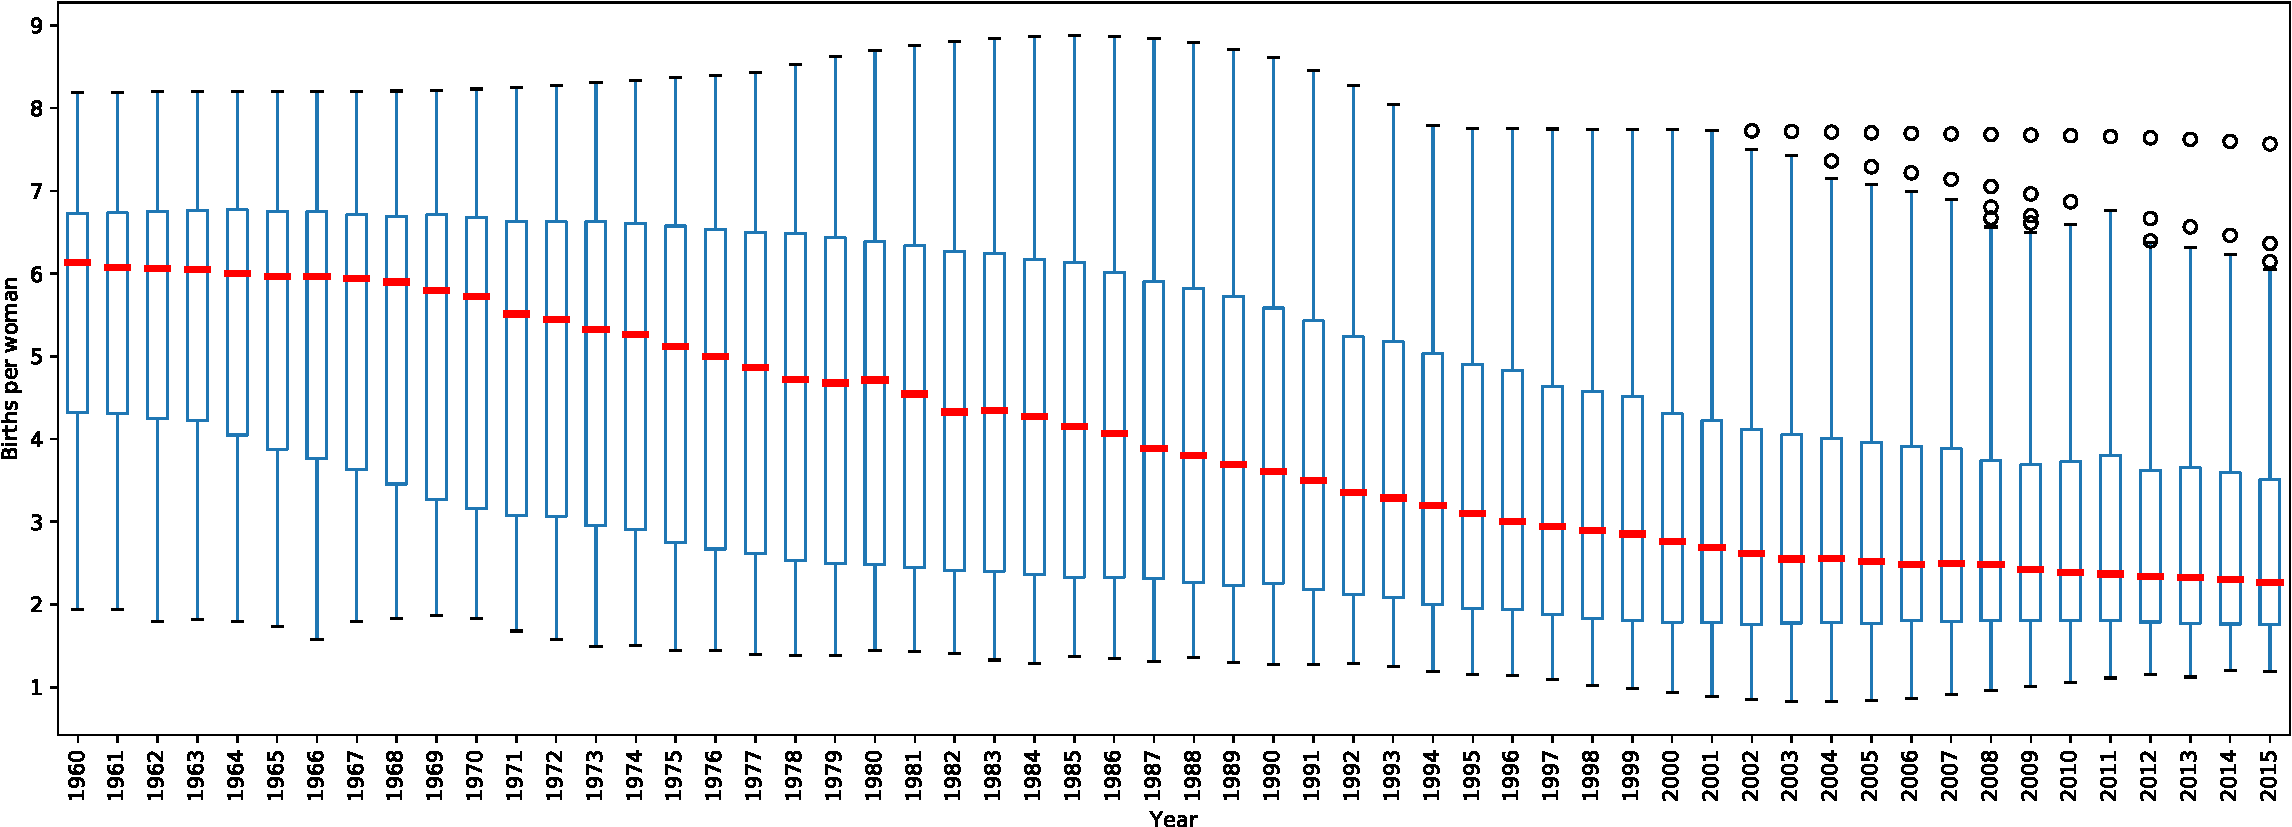
\includegraphics[width=\textwidth]{boxplot.pdf}
\end{center}

\end{frame}

%=============================================================================%
%=============================================================================%
\begin{frame}[fragile]
\frametitle{Reshaping data}

\begin{lstlisting}[style=python]
# Gather year columns into rows
df = pd.melt(data, 
             id_vars = ["CountryName", "Region", "IncomeGroup"], 
             var_name="Year", 
             value_name="Birth")
\end{lstlisting}

{\fontsize{8}{8}\selectfont
\begin{verbatim}
   CountryName                     Region          IncomeGroup  Year  Birth
0        Aruba  Latin America & Caribbean          High income  1960  4.820
1  Afghanistan                 South Asia           Low income  1960  7.450
2       Angola         Sub-Saharan Africa  Upper middle income  1960  7.379
3      Albania      Europe & Central Asia  Upper middle income  1960  6.489
4      Andorra      Europe & Central Asia          High income  1960    NaN 
\end{verbatim}}

\end{frame}

%=============================================================================%
%=============================================================================%
\begin{frame}[fragile]
\frametitle{Reshaping data}

\begin{lstlisting}[style=python]
# Spread rows into columns
df = pd.pivot_table(df, values="Birth", columns="CountryName", index="Year")
\end{lstlisting}

{\fontsize{7}{7}\selectfont
\begin{verbatim}
CountryName  Afghanistan  Albania  Algeria  American Samoa  Andorra  Angola  \
Year                                                                          
1960                7.45    6.489    7.524             NaN      NaN   7.379   
1961                7.45    6.401    7.573             NaN      NaN   7.388   
1962                7.45    6.282    7.614             NaN      NaN   7.396   
1963                7.45    6.133    7.646             NaN      NaN   7.402   
1964                7.45    5.960    7.665             NaN      NaN   7.406   

CountryName  Antigua and Barbuda  Arab World  Argentina  Armenia    ...     \
Year                                                                ...      
1960                       4.425    6.919764      3.109    4.550    ...      
1961                       4.386    6.941085      3.100    4.512    ...      
1962                       4.344    6.958855      3.089    4.435    ...      
1963                       4.299    6.970768      3.078    4.317    ...      
1964                       4.250    6.974893      3.068    4.161    ...      

CountryName  Zambia  Zimbabwe  
Year                           
1960          7.018     7.158  
1961          7.071     7.215  
1962          7.127     7.267  
1963          7.184     7.311  
1964          7.240     7.347 
\end{verbatim}}
\end{frame}

%=============================================================================%
%=============================================================================%
\begin{frame}[fragile]
\frametitle{Compare birth rates}

\begin{lstlisting}[style=python]
# Compare Malta vs United Kingdom
df.plot(y=["Malta", "United Kingdom"])
\end{lstlisting}

\vspace{-0.6cm}
\begin{center}
	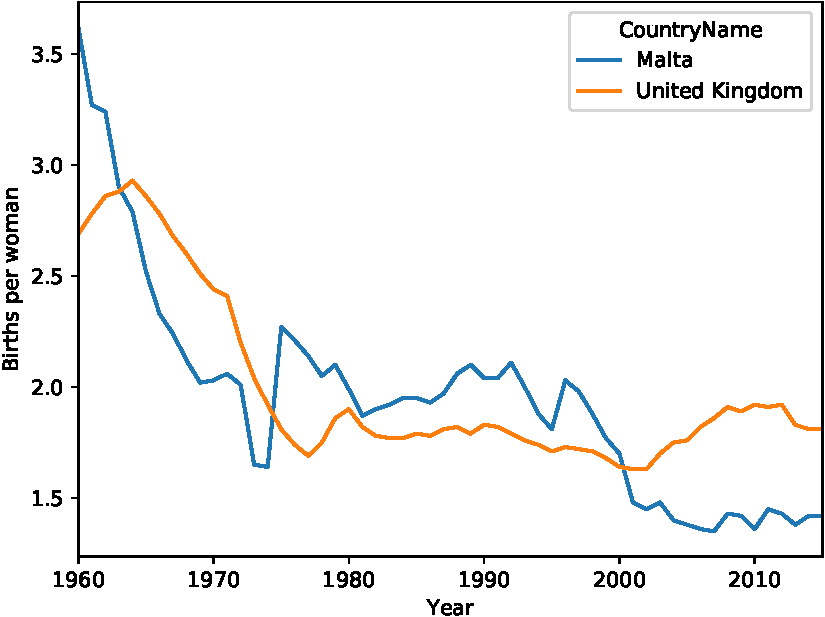
\includegraphics[width=.7\textwidth]{compare_births.pdf}
\end{center}

\end{frame}

%=============================================================================%
%=============================================================================%
% End of Document
%=============================================================================%
%=============================================================================%
\end{document}
